%%%%%%%%%%%%%%%%

% designed to be integrated with conceptual figure

%%%%%%%%%%%
\documentclass[border=0.2cm,11pt]{standalone}
\usepackage{tgheros}
\renewcommand*\familydefault{\sfdefault}%

\usepackage{tikz}
\usetikzlibrary{positioning,automata}
\usetikzlibrary{shapes}

\tikzset{>=latex} % for LaTeX arrow head
\usepackage{xcolor}

% taken from neural networks
\usepackage{amsmath} % for aligned
%\usepackage{amssymb} % for \mathbb
%\usepackage{etoolbox} % for \ifthen
\usepackage{listofitems} % for \readlist to create arrays
\usetikzlibrary{arrows.meta} % for arrow size
\usepackage[outline]{contour} % glow around text
\contourlength{1.4pt}

% using tableau 10 color palette: https://public.tableau.com/views/TableauColors/ColorPaletteswithRGBValues?%3Aembed=y&%3AshowVizHome=no&%3Adisplay_count=y&%3Adisplay_static_image=y

\definecolor{myblue}{RGB}{31,119,180}
\definecolor{myred}{RGB}{214,39,40}
\definecolor{mygreen}{RGB}{44,160,44}

% original colors defined by original author
\colorlet{myorange}{orange!70!red!60!black}
\colorlet{mydarkred}{red!30!black}
\colorlet{mydarkblue}{blue!40!black}
\colorlet{mydarkgreen}{green!30!black}
\tikzstyle{mynode}=[align=center, rounded corners, minimum height=1cm]
\tikzstyle{procs_ecolo}=[mynode, rectangle, fill=mygreen!30]
\tikzstyle{procs_evol}=[mynode, rectangle, fill=myred!30]
\tikzstyle{mechanisms}=[mynode, rectangle, thick, minimum width=3cm,fill=black!10]
\tikzstyle{patterns}=[mynode, circle, thick, fill=myblue!20]


% \tikzstyle{node}=[ultra thick,circle,minimum size=30,inner sep=2.,outer sep=0.6]
% \tikzstyle{node green}=[node,fill=mygreen]
% \tikzstyle{node blue}=[node,fill=myblue]
% \tikzstyle{node orange}=[node,orange!20!black,draw=myorange!30!black,fill=myorange!20]
% \tikzstyle{node red}=[node,fill=myred]
\tikzstyle{connect}=[thick,mydarkblue] %,line cap=round
\tikzstyle{connect arrow}=[-{Latex[length=4,width=3.5]},thick,mydarkblue,shorten <=0.5,shorten >=1]
 

% spacing nodes
% \tikzset{node distance = 0.5cm and 0.5cm}

\begin{document}

 
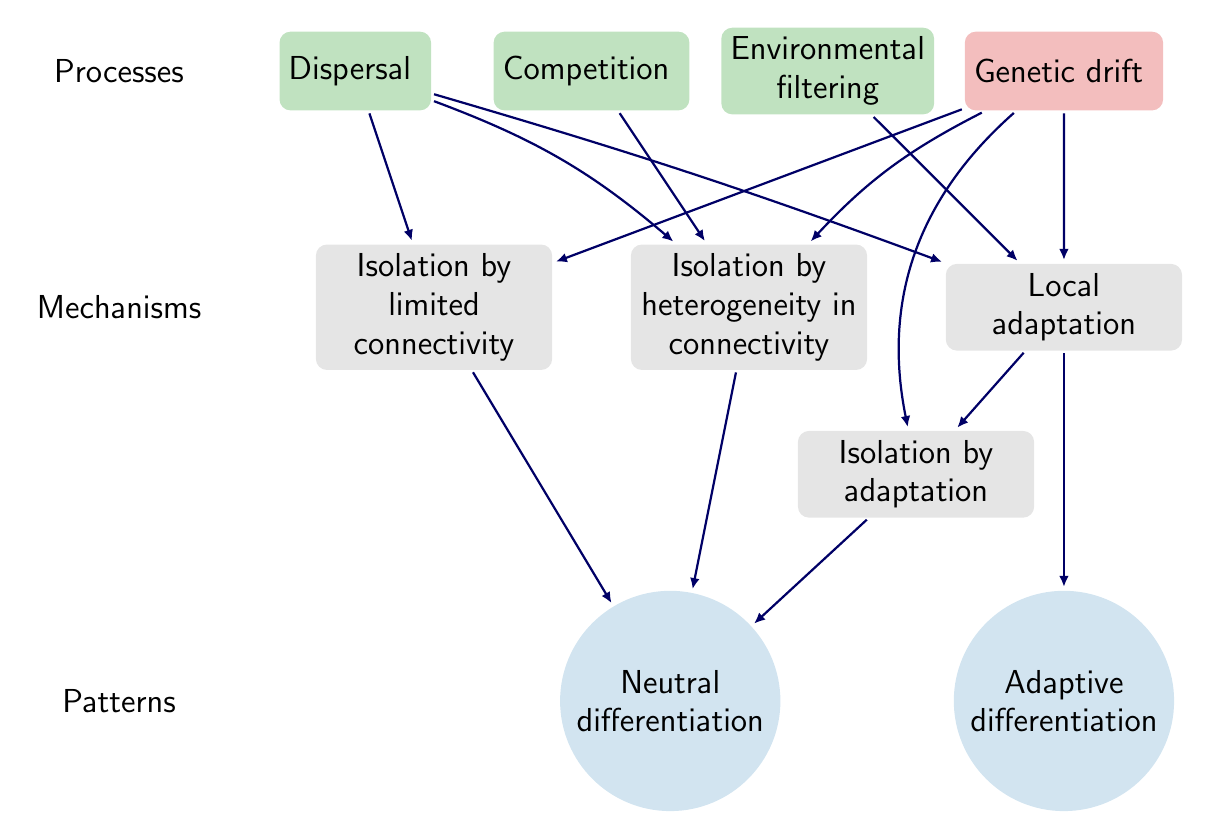
\begin{tikzpicture}[
    node distance=3cm,
    on grid,
    very thick,
    font=\large]
 
\node[] (procs) { Processes };
\node[] (mechs) [below=of procs] { Mechanisms };
\node[] (patt) [below=5cm of mechs]{ Patterns };

% Processes
\node[] (disp) [procs_ecolo, right=of procs]{ Dispersal };
\node[] (comp) [procs_ecolo, right=of disp]{ Competition };
\node[] (env) [procs_ecolo, right=of comp]{ Environmental\\filtering };
\node[] (drift) [procs_evol, right=of env]{ Genetic drift };

% Mechanisms
\node[mechanisms](l)[right=4cm of mechs]{Isolation by\\limited\\connectivity};
\node[mechanisms] (hc) [right=4cm of l]{ Isolation by\\heterogeneity in\\connectivity };
\node[mechanisms] (adapt) [right=4cm of hc]{ Local\\adaptation };
\node[mechanisms] (isol_adapt) [below right=of hc]{ Isolation by\\adaptation };

% Patterns
\node[patterns] (neutrdiff) [right=7cm of patt]{ Neutral\\differentiation };
\node[patterns] (adaptdiff) [right=5cm of neutrdiff]{ Adaptive\\differentiation };

\begin{scope} [connect arrow]  % now dashed is for the lines inside the scope
    % Processes to mechanisms
    \draw (comp) -- (hc); 

    \draw (drift) to (l); 
    \draw (drift) [bend right=10] to (hc); 
    \draw (drift) -- (adapt); 

    \draw (disp) -- (l); 
    \draw (disp) [bend left=10] to (hc); 
    \draw (disp)[bend left=2] to (adapt); 

    \draw (env) -- (adapt); 


    % mechs to mechs
    \draw (adapt) -- (isol_adapt)  ; 
    \draw (drift) to [bend right] (isol_adapt)  ; 


    % mech to patt
    \draw (l) -- (neutrdiff)  ; 
    \draw (hc) -- (neutrdiff)  ; 
    \draw (isol_adapt) -- (neutrdiff)  ; 
    \draw (adapt) -- (adaptdiff)  ; 

\end{scope}

\end{tikzpicture}
 
\end{document}